\documentclass[a4paper; 12pt]{article}

% global includes
\usepackage[polish]{babel}
\usepackage[utf8]{inputenc}
\usepackage{polski}
\usepackage{courier} %times, kurier
\usepackage{amsmath}
\usepackage{graphicx}
\usepackage{geometry}
\usepackage{indentfirst}
\usepackage{icomma}
\usepackage{booktabs}

\usepackage{listings}

% local includes
\usepackage[locale=FR]{siunitx}
\sisetup{per-mode=symbol-or-fraction}

\title{Temat 6: reakcja Biełousowa-Żabotyńskiego}
\author{Jakub Sawicki}
\date{\today}

\begin{document}
\renewcommand{\figurename}{Rys.}
\renewcommand{\tablename}{Tab.}
\renewcommand{\abstractname}{Abstrakt}

\maketitle

\section{Reakcja Biełousowa-Żabotyńskiego}

Jest to automat komórkowy, w~którym komórki mogą znajdować się w~następujących stanach:
\begin{itemize}
    \item \emph{Stan zdrowy --- 0}: nowy stan to $a/k_1+b/k_2$, gdzie $a$ to
        ilość zarażonych komórek wśród 8 sąsiadów a~$b$ to ilość chorych
        sąsiednich komórek.
    \item \emph{Stan chory --- $q$}: w~następnym kroku zdrowieje, tzn.~jej stan to 0.
    \item \emph{Stan zarażony --- 1 do $q-1$}: nowy stan to
        $s/(a+b+1)+g$, gdzie $s$ jest sumą stanów komórki i~sąsiadów, pozostałe
        oznaczenia jak dla komórki zdrowej.
\end{itemize}
Wartości $k_1$, $k_2$, $q$ oraz $g$ są stałe.
Występujące operacje dzielenia wykonywane są w~przestrzeni liczb całkowitych.

Na potrzeby symulacji ustawione zostały wartości $k_1 = 2$, $k_2 = 3$, $q = 10$
oraz $g = 3$.~\cite{hermetic}

\section{Analiza PCAM}

Analiza rozbita została na bloki: partition, communication, agglomeration oraz~mapping.~\cite{foster}

\subsection{Podział}
Komórki automatu umieszczone są w~dwuwymiarowej siatce, z~czego każda
komórka pamięta swój stan i~jest w~stanie przejść do następnego stanu bazując
na stanie komórek sąsiednich.
Podstawowym zadaniem będzie więc taka komórka.

Zakładając, że siatka jest kwadratowa mamy $n^2$ takich zadań. 
Każde zadanie przechowuje dane w~postaci jednej liczby naturalnej O(1) i~ma
stały czas wykonania O(1) (przy zaniedbaniu komunikacji).

\subsection{Komunikacja}
Wymiana komunikatów następować musi pomiędzy sąsiednimi komórkami.
Każda komórka musi dowiedzieć się o~stanie swoich 8 sąsiadów.

Daje nam to w~sumie $8 n^2$ komunikatów o~wielkości 1 (umownie) do wysłania na
krok czasowy.

\subsection{Aglomeracja}
Optymalnym pod względem redukcji komunikacji jest podział kolumnowy.
\begin{lstlisting}[basicstyle=\ttfamily]
1122334455
1122334455
1122334455
...       
1122334455
\end{lstlisting}
Komunikacja zachodzi w~tym przypadku jedynie pomiędzy sąsiednimi kolumnami.
Daje to redukcję w ilości komunikatów do $2t$, gdzie $t$ jest ilością bloków. 
Każdy komunikat jest też w~tym przypadku większy, ma rozmiar $n$.

\subsection{Mapowanie}
W~zależności od tego ile jest dostępnych procesorów/wątków, na tyle bloków
można podzielić siatkę. 
Dzięki temu obliczenia dla poszczególnych bloków nie będą sobie wchodzić
w~drogę.
Warto też zadbać o lokalność komunikacji umieszczając sąsiednie bloki na
fizycznie bliskich procesorach.

\section{Implementacja}

Kod programu znajduje się pod \texttt{github.com/jswk/AR/lab1/CA.c}.
Został on napisany w~C z~wykorzystaniem MPI do komunikacji.

Ustawienie stałej \texttt{DEBUG} pozwala wypisywać stan symulacji na
standardowe wyjście.
Na podstawie pliku wyjścia za pomocą skryptu \texttt{process.sh} możliwe jest
wygenerowanie wizualizacji procesu.

Struktury wygenerowane przez program widoczne są na Rys.~\ref{fig:automat}.

\begin{figure}[b!]
    \centering
    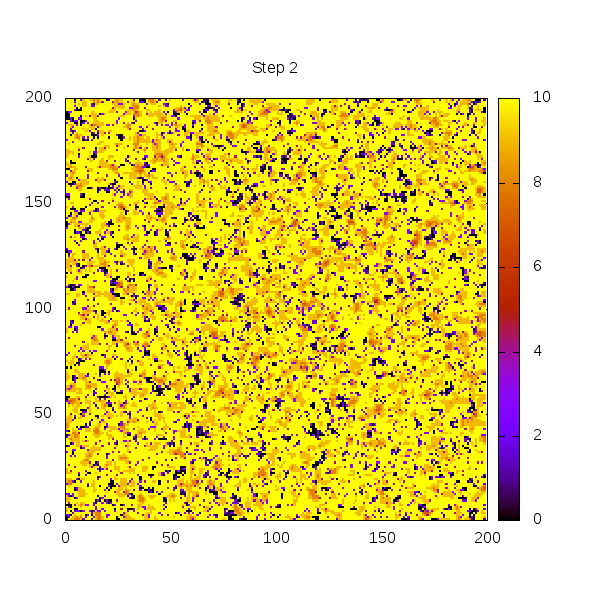
\includegraphics[width=.45\textwidth]{fig/plot_2.png}
    \hfill
    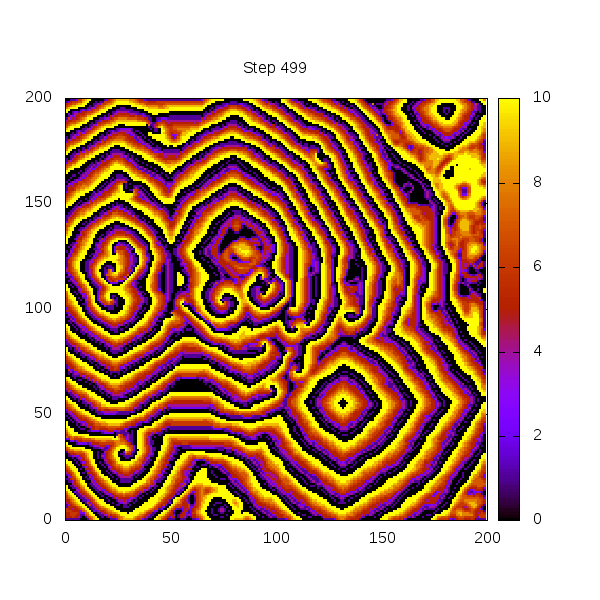
\includegraphics[width=.45\textwidth]{fig/plot_499.png}
    \caption{Wykresy pokazują stan automatu dla 2. i~499. iteracji.
             Kolorem oznaczony jest stan poszczególnych komórek.
             Zobaczyć można wykształcenie zorganizowanych struktur z~początkowo
             losowego stanu.}
    \label{fig:automat}
\end{figure}

\section{Wydajność}

Program uruchomiony został na klastrze Zeus.
Pomiary obejmowały różne ilości aktywnych procesorów, od 1 do 24 (dwa node'y po 12 rdzeni).

Przeprowadzone zostało kilka pomiarów.
Pierwszy dla wielkości problemu $n = 200$.
Następnie dla $n = 1000$ oraz dla skalowanego problemu (ok. $10^6$ komórek na procesor).

Wyniki dla $n = 200$ przedstawione zostały na Rys.~\ref{fig:n200}.
Problem ten był zbyt mały dla ilości procesorów większej niż 5--6.
Dla większych ilości procesorów narzut komunikacyjny prowadził do zmniejszenia
efektywności.

Dla $n = 1000$ wyniki przedstawione są na Rys.~\ref{fig:n1000}.
Tutaj większa ilość procesorów daje większy wzrost wydajności, efektywność nie
opada tak szybko jak w~przypadku poprzednim.

Dla problemu skalowanego wyniki są na Rys.~\ref{fig:s1000}.
Rozmiar problemu skalowany był w~taki sposób, aby zawsze na jeden procesor
przypadało ok. $10^6$ komórek.


\begin{figure}
    \centering
    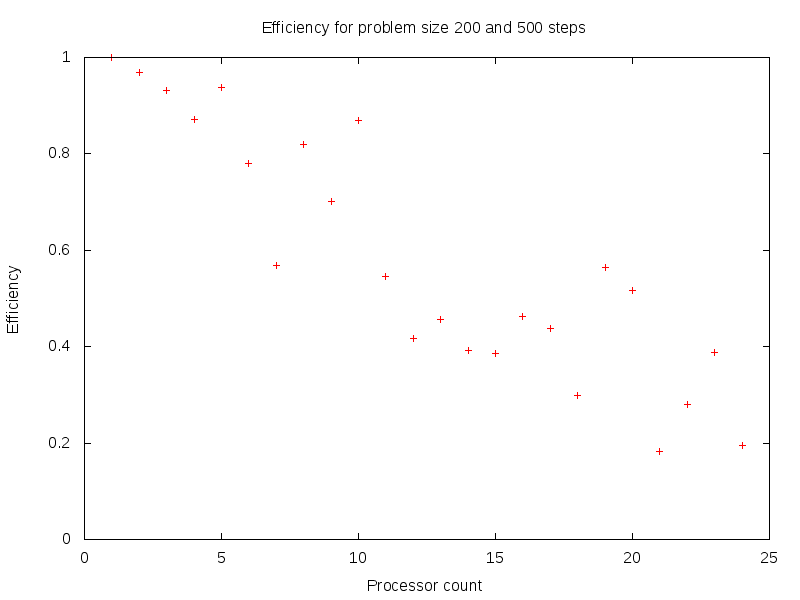
\includegraphics[width=.45\textwidth]{fig/size_200_e.png}
    \hfill
    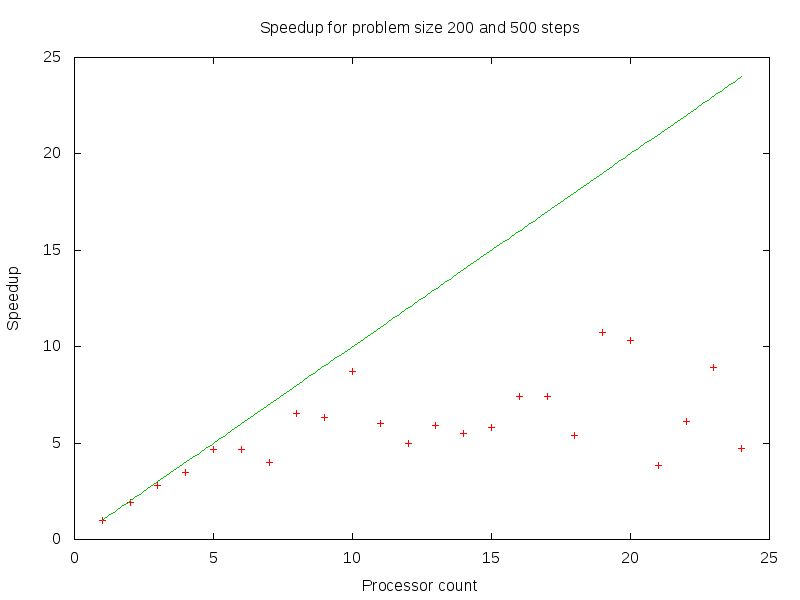
\includegraphics[width=.45\textwidth]{fig/size_200_s.png}
    \caption{Wykresy pokazują efektywność oraz przyspieszenie dla problemu
        wielkości $n = 200$.}
    \label{fig:n200}
\end{figure}

\begin{figure}
    \centering
    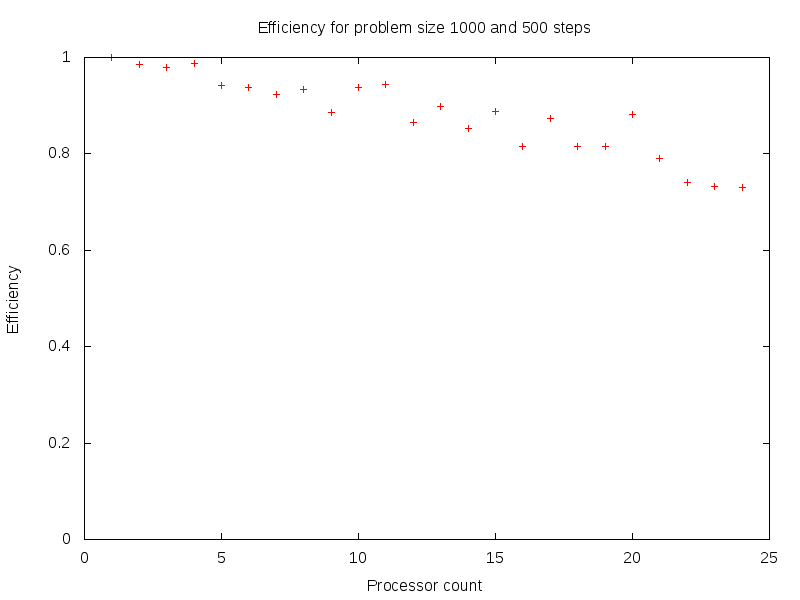
\includegraphics[width=.45\textwidth]{fig/size_1000_e.png}
    \hfill
    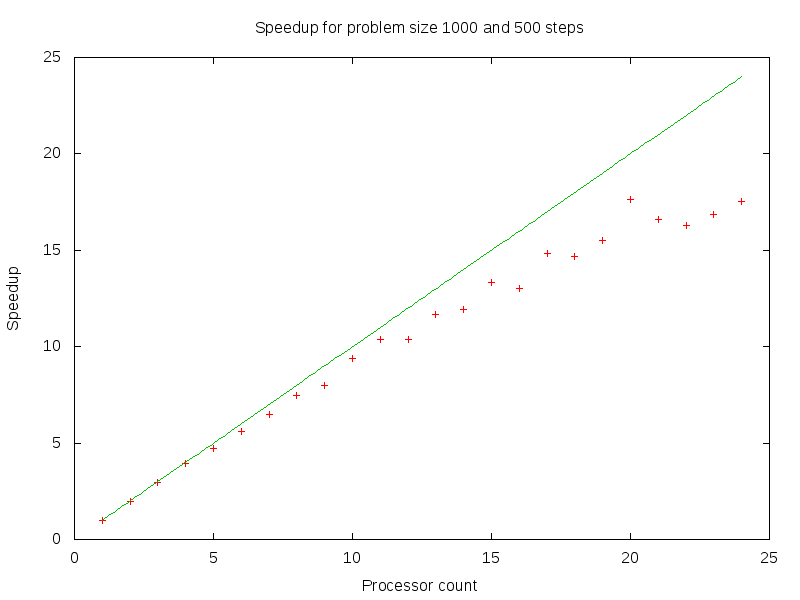
\includegraphics[width=.45\textwidth]{fig/size_1000_s.png}
    \caption{Wykresy pokazują efektywność oraz przyspieszenie dla problemu
        wielkości $n = 1000$.}
    \label{fig:n1000}
\end{figure}

\begin{figure}
    \centering
    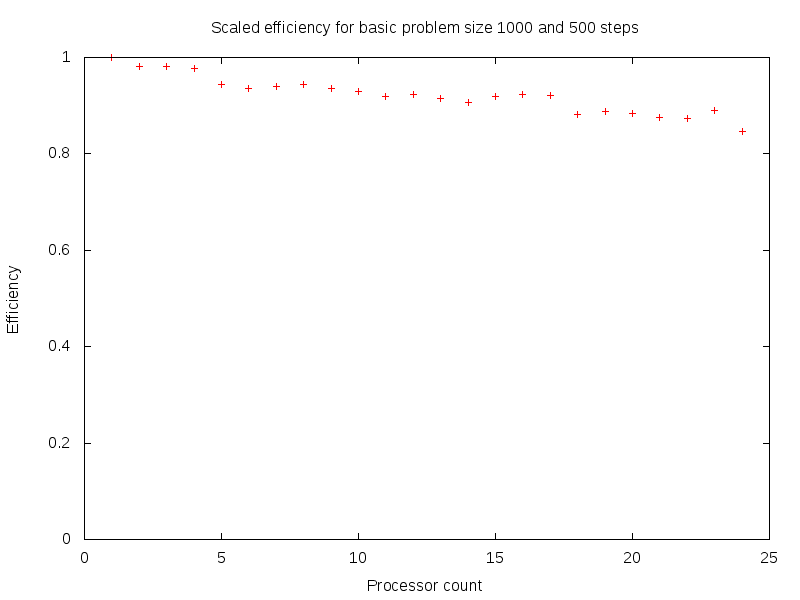
\includegraphics[width=.45\textwidth]{fig/scaled_1000_e.png}
    \hfill
    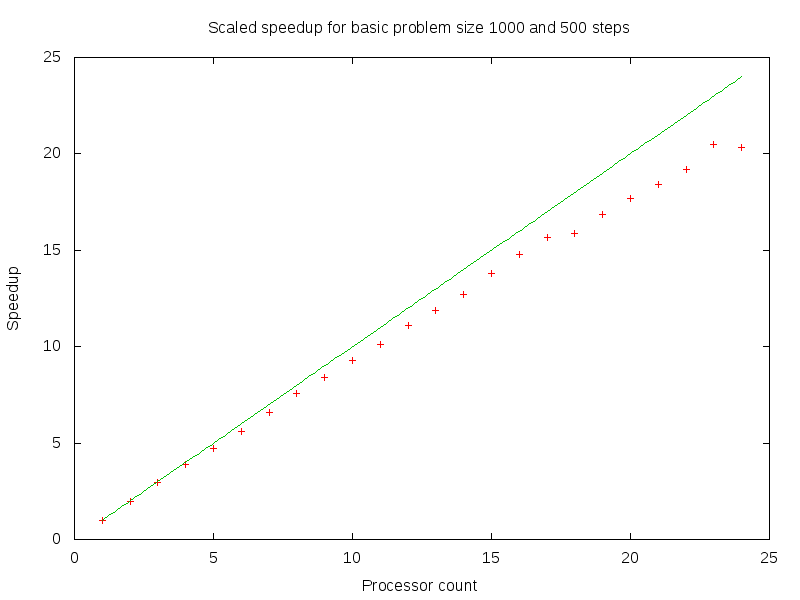
\includegraphics[width=.45\textwidth]{fig/scaled_1000_s.png}
    \caption{Wykresy pokazują efektywność oraz przyspieszenie dla skalowanego
        problemu, ok. $10^6$ komórek na procesor.}
    \label{fig:s1000}
\end{figure}


\begin{thebibliography}{9}
    \bibitem{foster}
        I.~Foster: \emph{Designing and Building Parallel Programs}
        \texttt{http://www.mcs.anl.gov/dbpp/} dostęp 2015.10.14
    \bibitem{hermetic}
        Hermetic Systems: \emph{Five Cellular Automata: The Belousov-Zhabotinsky Reaction}
        \texttt{http://www.hermetic.ch/pca/bz.htm} dostęp 2015.03.04
\end{thebibliography}

\end{document}
